\documentclass[10pt]{article}
\usepackage[english]{babel}
\usepackage[utf8]{inputenc}
\usepackage[T1]{fontenc}
\usepackage[a4paper,top=2cm,bottom=2cm,left=3cm,right=3cm,marginparwidth=1.75cm]{geometry}

% Useful packages
\usepackage{amsmath}
\usepackage{float}
\usepackage{listings}
\usepackage{graphicx}
\usepackage{subcaption}
\usepackage{graphicx}
\usepackage{authblk}
\usepackage{amsmath}
\usepackage{multirow}

\usepackage[colorlinks=true, allcolors=blue]{hyperref}
\usepackage[acronym]{glossaries}

\usepackage{listings}
\usepackage{amssymb}
\usepackage[usenames,dvipsnames]{color}    

\lstset{ 
  language=R,                     % the language of the code
  basicstyle=\ttfamily, % the size of the fonts that are used for the code
  numbers=left,                   % where to put the line-numbers
  numberstyle=\color{Blue},  % the style that is used for the line-numbers
  stepnumber=1,                   % the step between two line-numbers. If it is 1, each line
                                  % will be numbered
  numbersep=5pt,                  % how far the line-numbers are from the code
  backgroundcolor=\color{white},  % choose the background color. You must add \usepackage{color}
  showspaces=false,               % show spaces adding particular underscores
  showstringspaces=false,         % underline spaces within strings
  showtabs=false,                 % show tabs within strings adding particular underscores
  frame=single,                   % adds a frame around the code
  rulecolor=\color{black},        % if not set, the frame-color may be changed on line-breaks within not-black text (e.g. commens (green here))
  tabsize=2,                      % sets default tabsize to 2 spaces
  captionpos=b,                   % sets the caption-position to bottom
  breaklines=true,                % sets automatic line breaking
  breakatwhitespace=false,        % sets if automatic breaks should only happen at whitespace
  keywordstyle=\color{RoyalBlue},      % keyword style
  commentstyle=\color{YellowGreen},   % comment style
  stringstyle=\color{ForestGreen}      % string literal style
} 
\usepackage[backend=biber,style=apa6,sorting=ynt]{biblatex}
\addbibresource{references.bib}

\begin{document}
\begin{titlepage}
    \begin{center}
        \vspace*{1cm}
            
        \Huge
        \textbf{Project On Time Series}
            
        \vspace{0.5cm}
        \LARGE
        \textbf{TSM\_AnSeqDa}
        
        \vspace{0.5cm}
        \LARGE
        \textbf{Group AF}

        \vspace{1cm}
        \Large
        06.12.2022
        

        \Large
        \vspace{2.5cm}
        \textbf{Supervisor}\\ Giorgio Corani

        \vspace{0.5cm}
        \textbf{Authors}\\
        Willi Adrian\\
        Bär Florian
            
  
            
        \vfill
            
            
        
    
        
            
            
        \vspace{0.8cm}
            
        
\includegraphics[width=0.5\textwidth]{mse.png}
            
        \Large
        Lucerne University of\\
        Applied Sciences and Arts\\
        
            
    \end{center}
\end{titlepage}




\section{Introduction}
This project focuses on the analysis of a specific time series of the M3-Competition \autocite{Makridakis1982-kv}. The name of the time series, which will be further analyzed is: "\textbf{OECD ECONOMIC OUTLOOK - SWITZERLAND Gross Domestic Product- Volume Indeces}" containing quaterly index volume values from the swiss gross domestic product (GDP). The GDP is a monetary measure of the market value of all the goods and services produced and sold in a specific time period by countries.

\section{Exploratory analysis}
The time series is splitted into a training and a test set, where the training set contains values from 1980 until 1990 whereas the test set contains values from the years 1991 and 1992. 

\begin{figure}[ht!]
\centering
\begin{subfigure}{.4\textwidth}
  \centering
  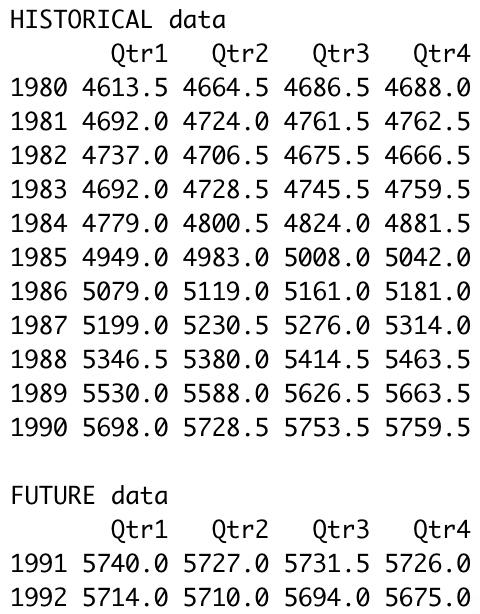
\includegraphics[width=0.9\linewidth]{img/m3data.png}
  \caption{Historical and future data}
  \label{fig:data_points}
\end{subfigure}%
\begin{subfigure}{.6\textwidth}
  \centering
  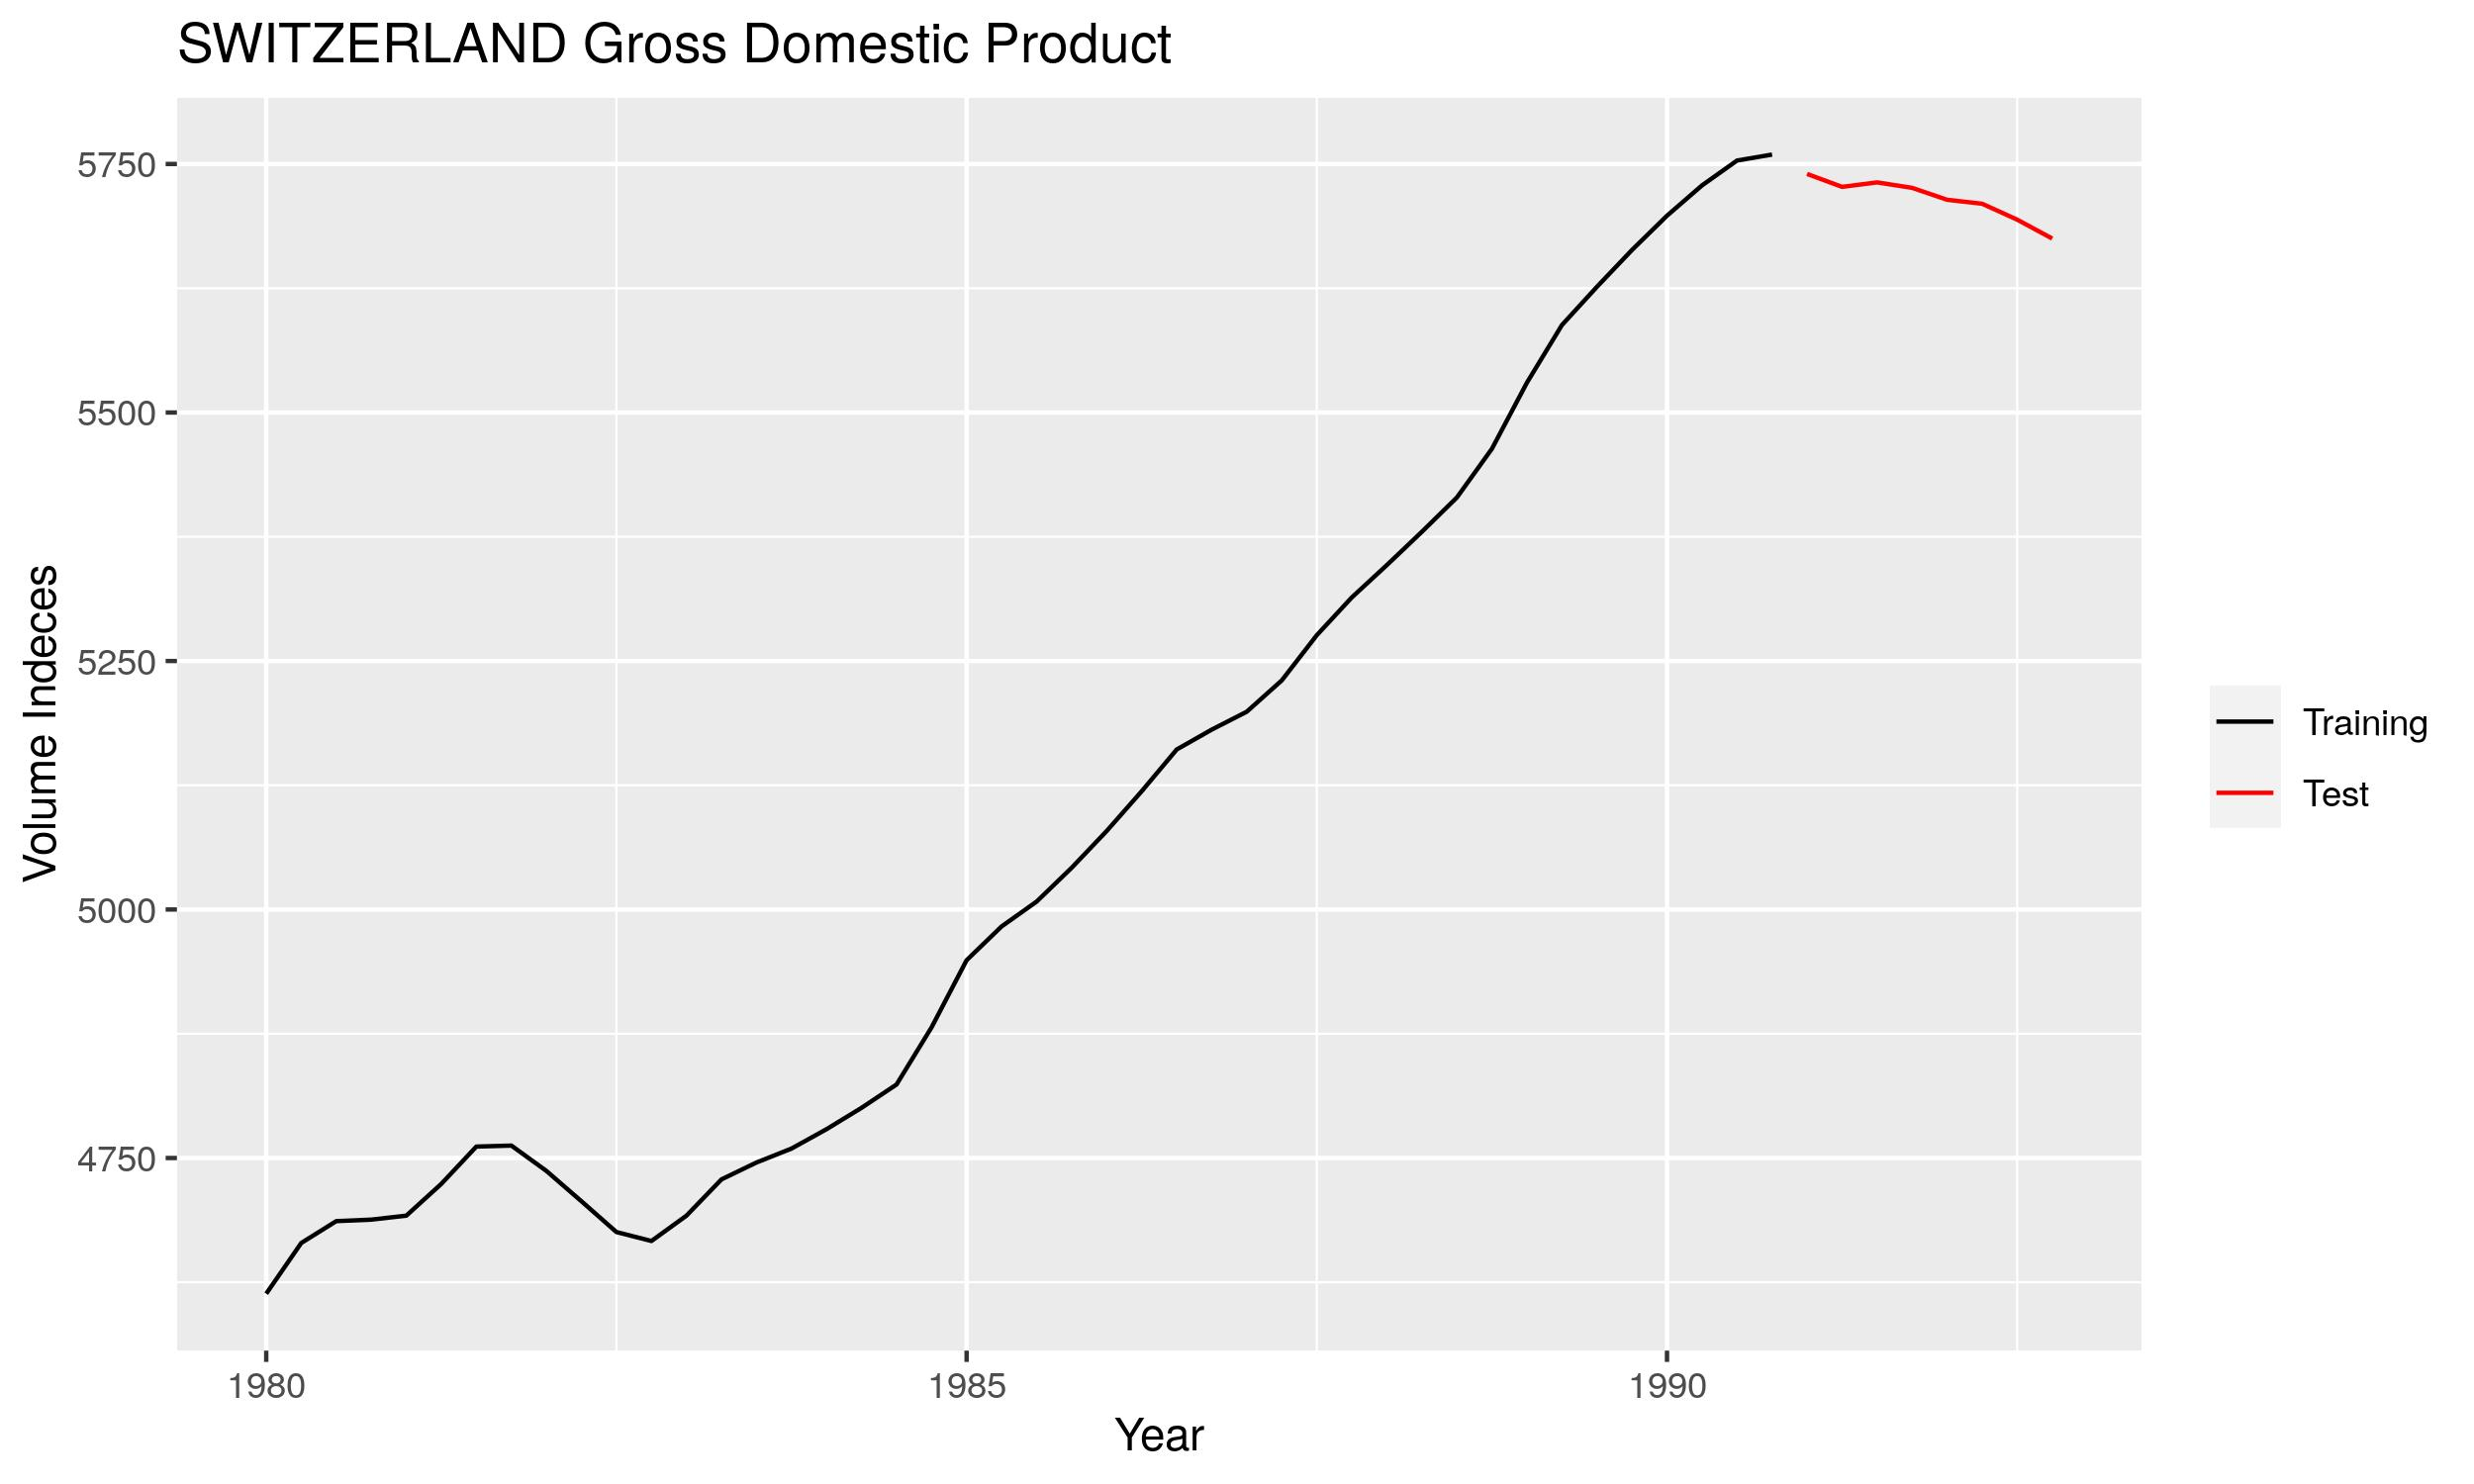
\includegraphics[width=1\textwidth]{img/autoplot.jpeg}  %the image must be resized or scaled if needed
  \caption{Autoplot of the dataset}
  \label{fig:autoplot}
\end{subfigure}
\caption{Overview of the time series}
\label{fig:overview_plots}
\end{figure}
\noindent The values of the \textbf{training data} are rising steadily after a pullback in the years 1981 and 1982 which was caused by tight monetary policy in an effort to fight mounting inflation \autocite{Sablik_undated-bb}. From the plots in \autoref{fig:seasonal_plots}, there is no obvious seasonality visible in this dataset. Moreover, we used the \textit{tbats()} \autocite{Hyndman2013-za} function from the \textit{forecasting} package, which confirms our assumption. It stands out that by the end of the training dataset, starting from Qrt2 1990, the trend stops and will then decrease in the test data.

\begin{figure}[ht!]
\centering
\begin{subfigure}{.5\textwidth}
  \centering
  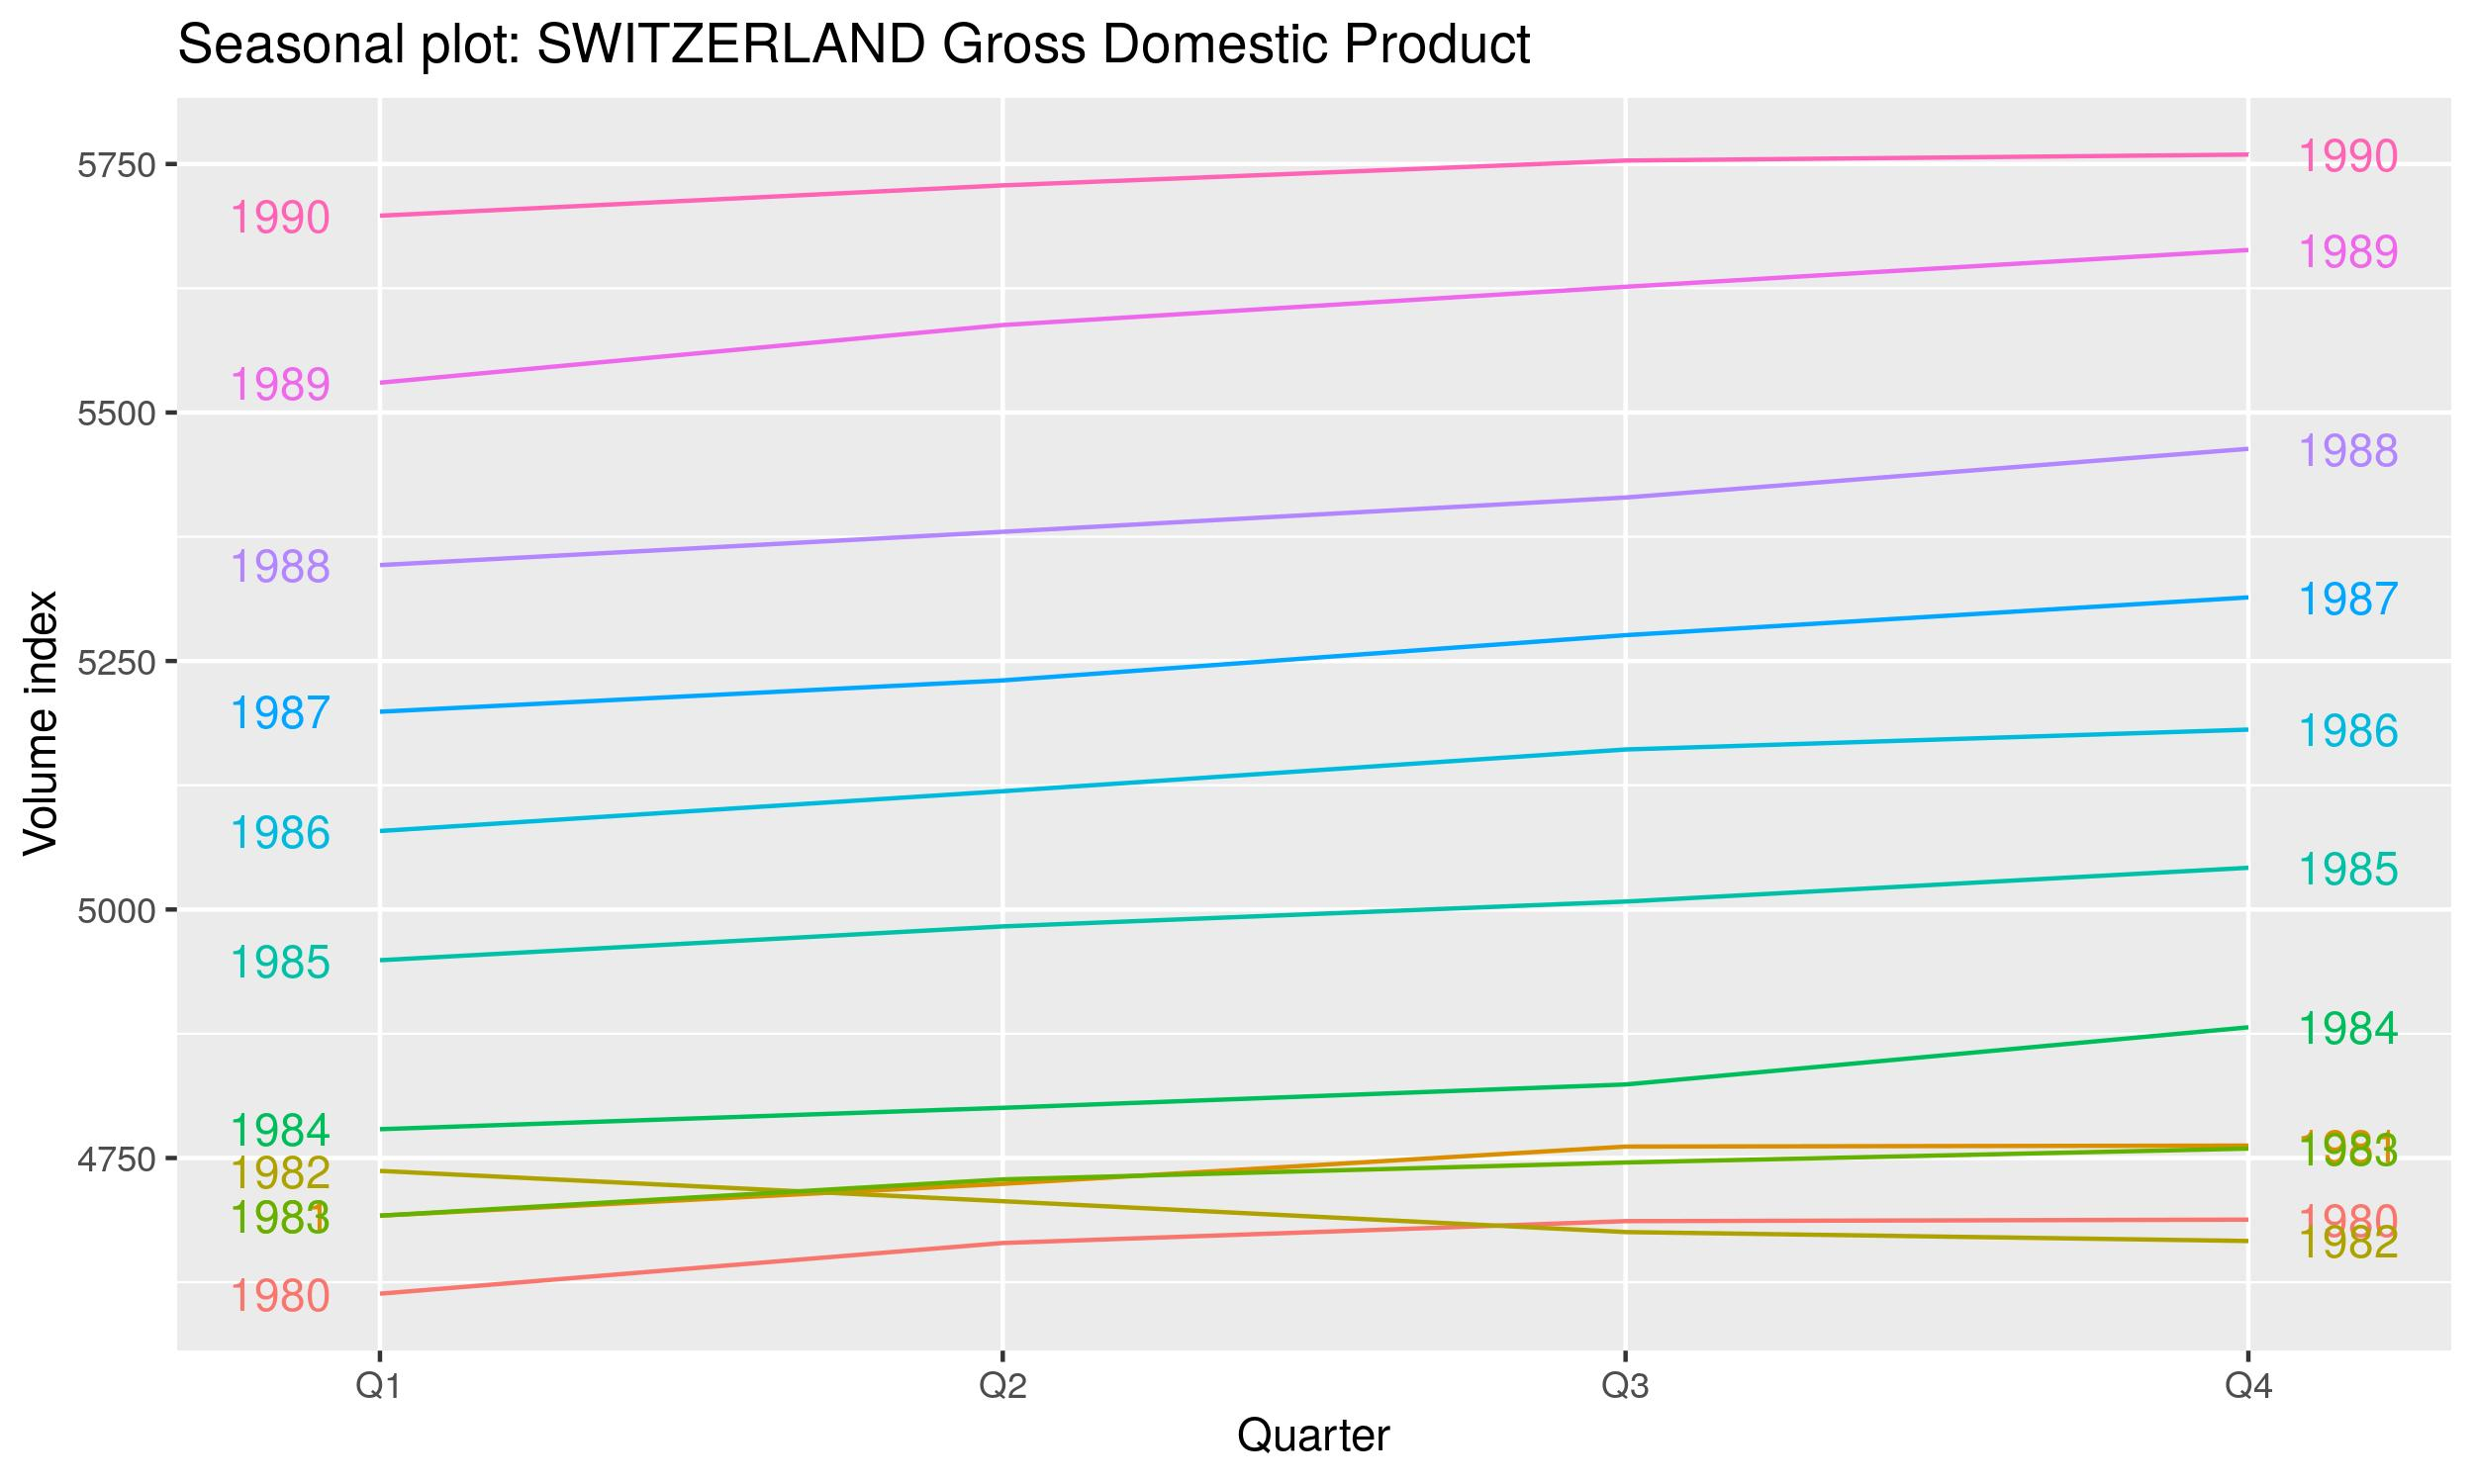
\includegraphics[width=1\linewidth]{img/seasonal.jpeg}
  \caption{Seasonal plot per year}
  \label{fig:seasonal_plot_per_year}
\end{subfigure}%
\begin{subfigure}{.5\textwidth}
  \centering
  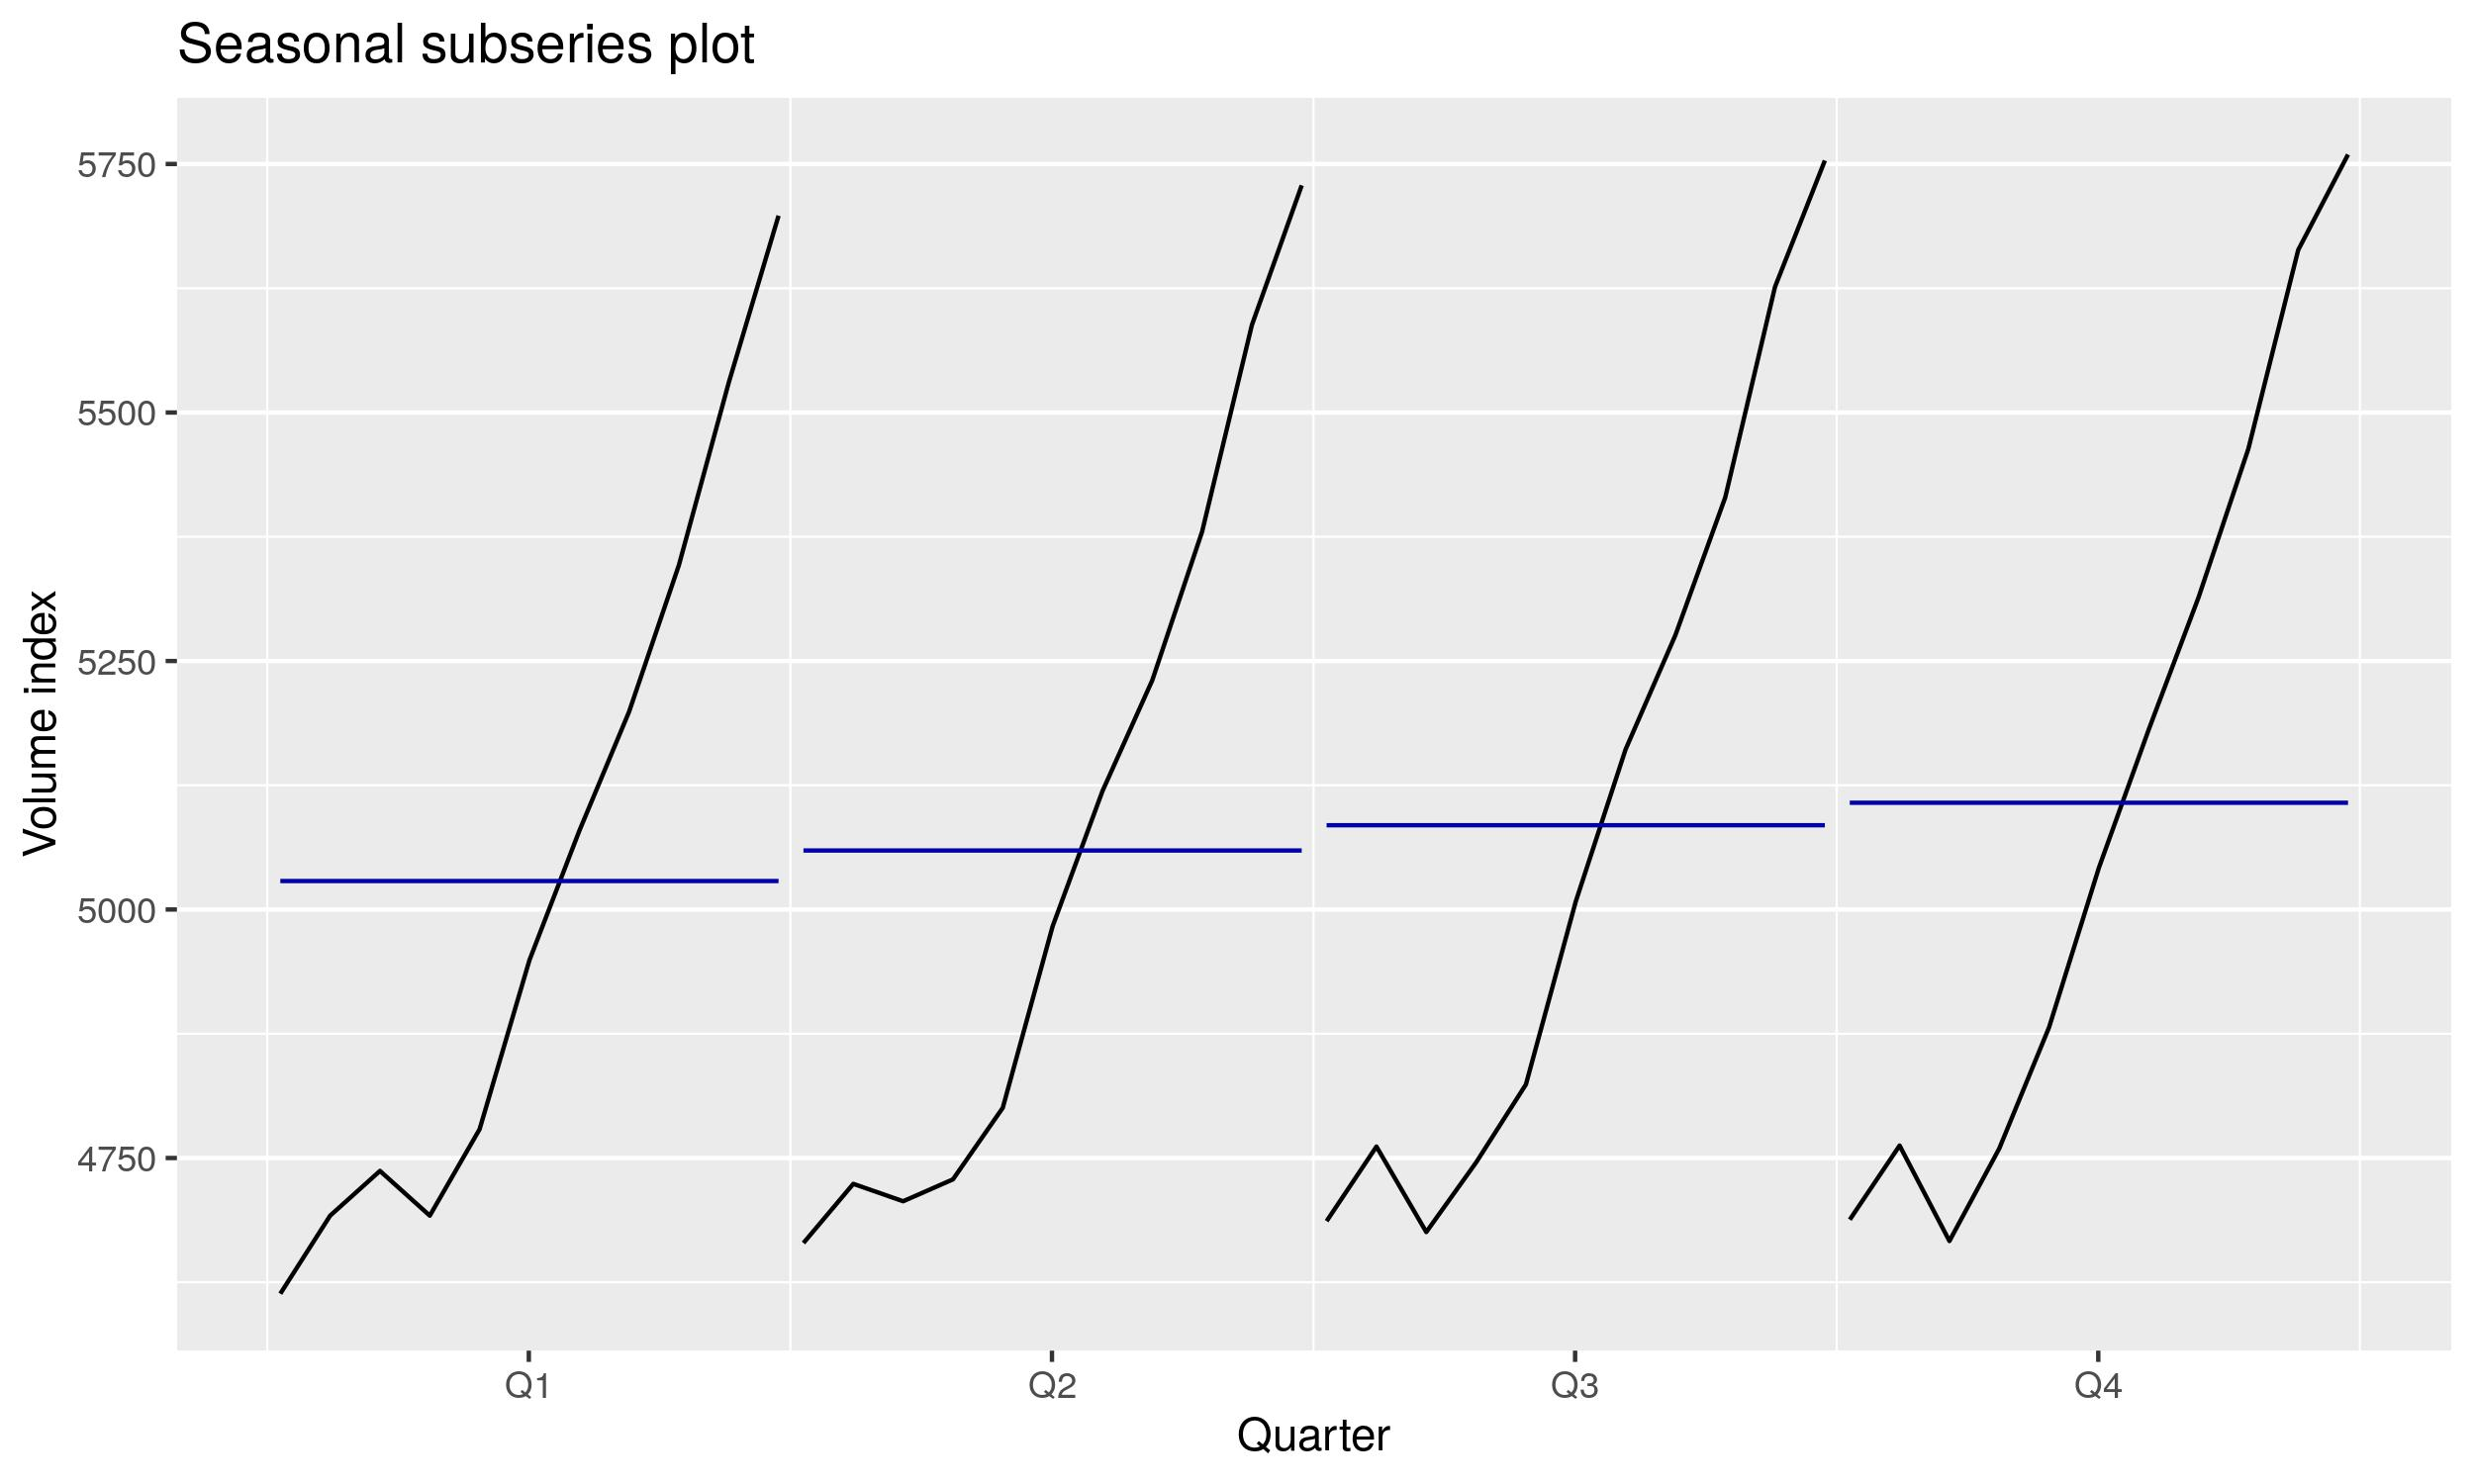
\includegraphics[width=1\linewidth]{img/subseriesplot.jpeg}
  \caption{Seasonal subplot for the training data}
  \label{fig:seasonal_sub_plot}
\end{subfigure}
\caption{The seasonal plots for the training data}
\label{fig:seasonal_plots}
\end{figure}
\clearpage
\noindent The autocorrelation analysis of the training data shows significant autocorrelation with lower lags. This is clearly visible in both, the lag plot and the ACF plot in \autoref{fig:autocorrelation_and_lag_plot}. Therefore, the training data is not white noise.
\begin{figure}[ht!]
\centering
\begin{subfigure}{.5\textwidth}
  \centering
  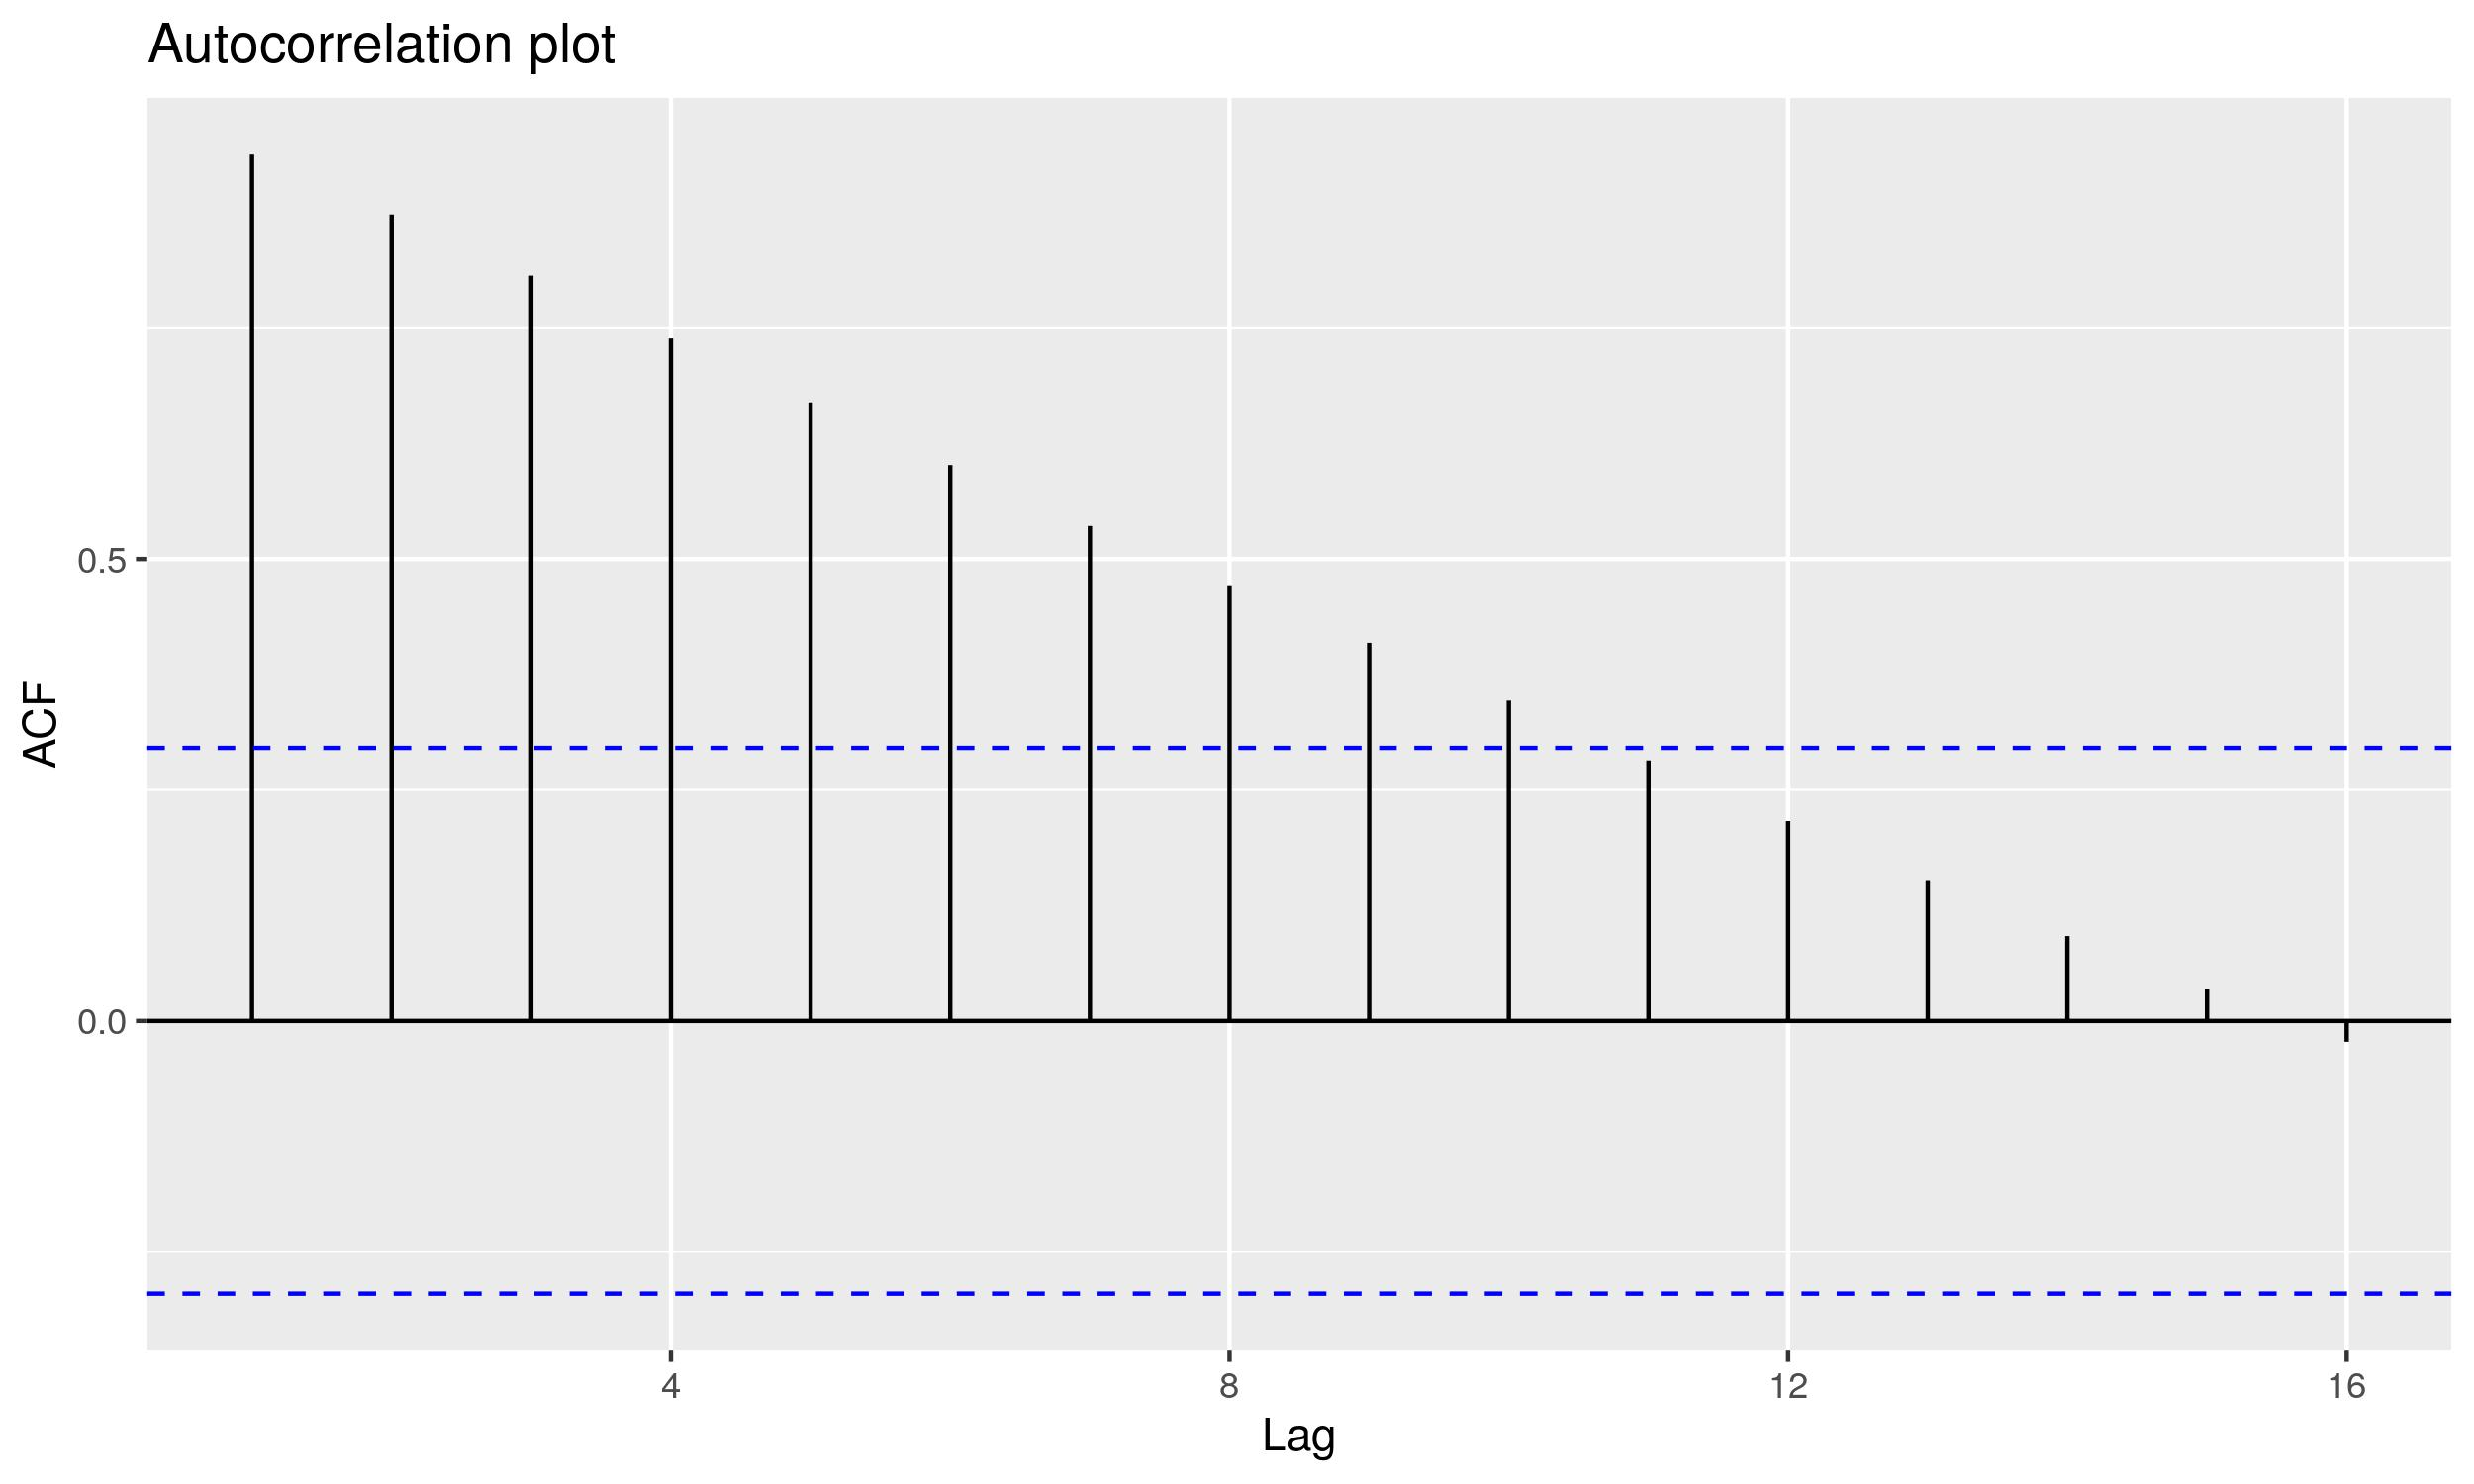
\includegraphics[width=1\linewidth]{img/autocorrelation.jpeg}
  \caption{Autcorrelation plot}
  \label{fig:autocorrelation}
\end{subfigure}%
\begin{subfigure}{.5\textwidth}
  \centering
  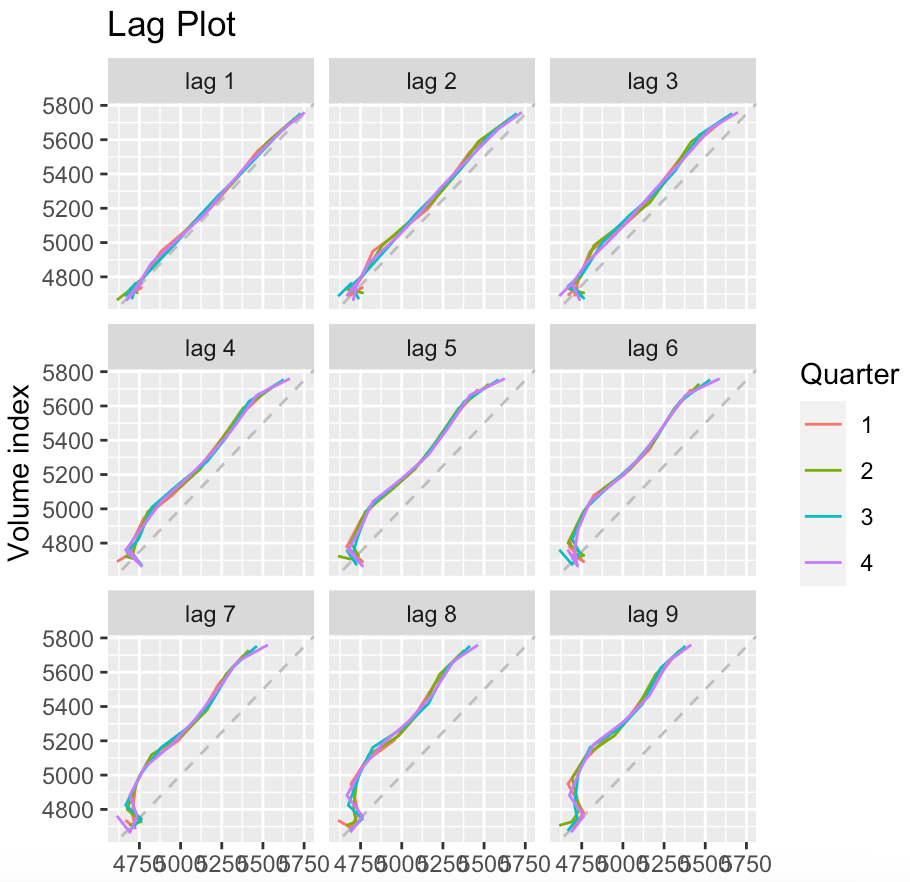
\includegraphics[width=1\linewidth]{img/lagplot.png}
  \caption{Lag plots for lag = $1, \dots, 9$}
  \label{fig:lag_plot}
\end{subfigure}
\caption{The seasonal plots for the training data}
\label{fig:autocorrelation_and_lag_plot}
\end{figure}
\section{Indicators}
We used a combination of two different indicators, both having different properties to interpret the performance of our models. This serves on the one hand to have an easy understandable metric and on the other hand to have a weighted importance of errors. Therefore, we have chosen the following metrics:
\begin{itemize}
    \item \textbf{MAE\footnote{Mean Absolut Error} $ = \frac{\sum _{i=1}^{n}\left|y_{i}-x_{i}\right|}{n}  $}
    \begin{itemize}
		\item Easy to interpret
		\item Scale dependency can be disregarded, because we focus only on one time series
		\item Very robust against outliers
	\end{itemize}
    \item \textbf{RSME\footnote{Root Mean Squared Error - suggested by \url{https://stats.stackexchange.com/questions/554432}} $ = \sqrt {\frac{1}{N} \sum_{i=1}^{N} (\hat{y_{i}} - y_{i})^2} $}
    \begin{itemize}
		\item exponentially more weight on large error by squaring it
		\item easy interpretable as there is a direct relationship with the correlation coefficient
	\end{itemize}
\end{itemize}
% see https://medium.com/human-in-a-machine-world/mae-and-rmse-which-metric-is-better-e60ac3bde13d
% https://en.wikipedia.org/wiki/Root-mean-square_deviation

\subsection{Targets for the indicators}
% https://stats.oecd.org/glossary/detail.asp?ID=2875
Unfortunately, it is not clear in which unit the data is provided in the \textbf{M3comp} package. Therefore, we assume that the used unit will be in million USD. As the \textit{volume index} is an absolute measurement of the GDP, we define the target for our indicator as $\pm 1\%$ of our last data point from the training data set. This leads to the following values:
$$\text{MAE} = 5759.5 * 0.01 \approx 57.595 $$
$$\text{RSME} = \sqrt{\frac{\sum^{N}_{i = 1} \left| y^i - \hat{y}^i \right|}{N}} \approx 60 $$
Given the fact, that the \textbf{RSME} will give larger deviations on the real value a bigger penatly, we increased the target for the \textbf{RSME} to a value of 60.

\section{Simple model}
The GDP of a country shows how successful the economy of a country is. Therefore global crises and the underlying economic cycles have a huge effect on the GDP. As we observed in the last 3 years, an extremely big number of factors with randomness and unexpected circumstances can have a big impact on a country's GDP. This makes a prediction of economic numbers extremely hard, as there is almost no way to identify all needed predictors. We decided therefore to use a random walk with drift, which is the best matching baseline model to predict these values. The drift makes sure to include the previous year's increase in the GDP.

\vspace{.5cm}
\begin{figure}[h]
\begin{minipage}{.7\textwidth}  %listing bloc will have 50% of the line width 
\lstset{linewidth = 6cm, breaklines=true} %set your listing lines widths, and set breaklines to true
\begin{lstlisting}[basicstyle=\footnotesize,numbers=none]
Ljung-Box test

data:  Residuals from Random walk with drift
Q* = 39.133, df = 7, p-value = 1.844e-06

Model df: 1.   Total lags used: 8
\end{lstlisting}
\label{lst:rw_drift}
\end{minipage}
\qquad %space between listing bloc and the figure
\begin{minipage}{0.6\textwidth} %figure will have the remaning 40% of the line width
    \centering
    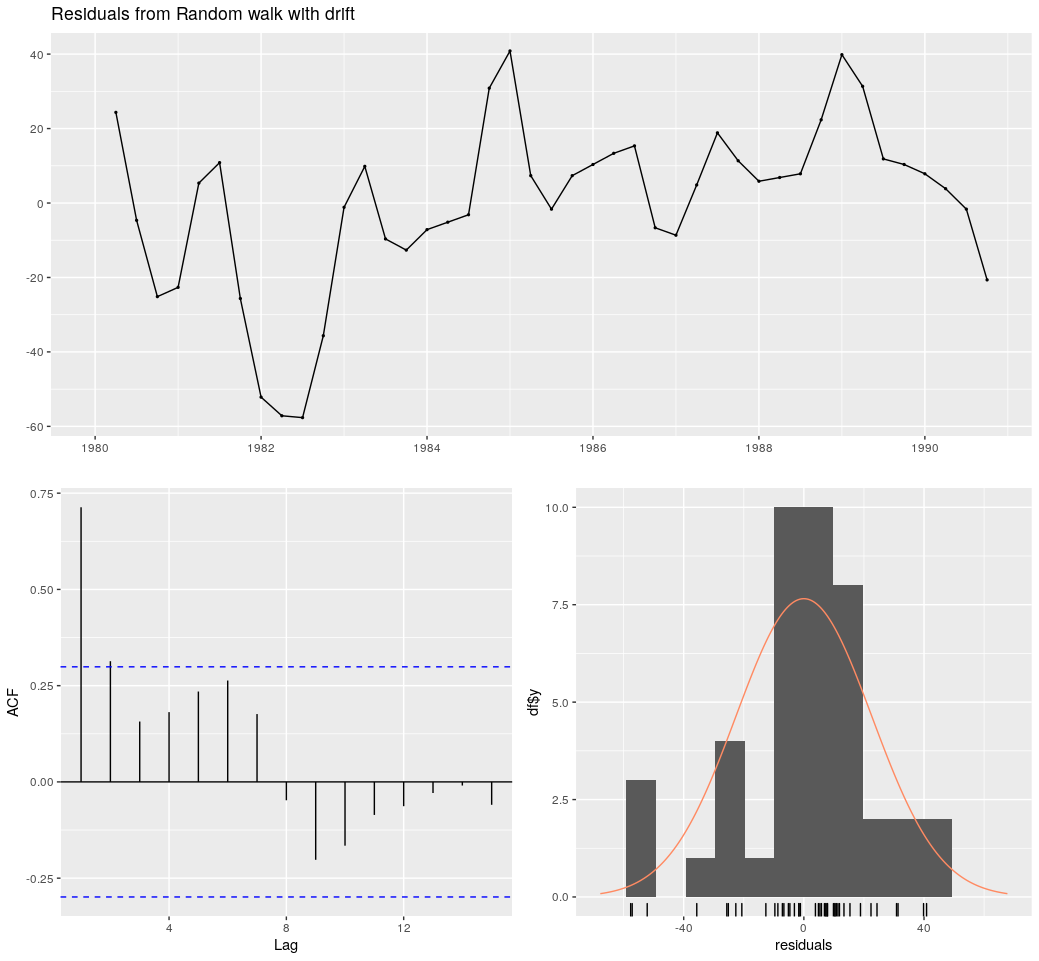
\includegraphics[width=0.9\textwidth]{img/check_resid_simple_model.png}
    \caption{Residual analysis of the simple model}
    \label{fig:resid_simple}
\end{minipage}
\end{figure}
\noindent The Ljung-Box test p-value with a value of 1.844e-06 shows a high correlation between the residuals and indicate that the residuals are not white noise. This is as well visible in \autoref{fig:resid_simple} as there is a visible auto correlation between the lags. This can't be explained at this point. We assume, that this simple model does not have the capacity and capability to train the underlying patterns of this data set.
\begin{table}[ht]
\centering
\begin{tabular}{rrrrrrrrr}
  \hline
 & ME & \textbf{RMSE} & \textbf{MAE} & MPE & MAPE & MASE & ACF1 & Theil's U \\ 
  \hline
Training set & 0.00 & 22.32 & 16.69 & -0.01 & 0.34 & 0.14 & 0.71 & N/A \\ 
  Test set & -95.00 & 100.96 & 95.00 & -1.66 & 1.66 & 0.80 & 0.20 & 13.28 \\ 
   \hline
\end{tabular}
\caption{Accuracy table of the random walk with drift}
\label{tab:resid_simple}
\end{table}

\noindent Furthermore, the accuracy in \autoref{tab:resid_simple} shows, that the \textbf{MAE} and the \textbf{RSME} deviate quite heavily between the training and the test set. This indicates a high overfit of the model to the training data, even though the model is not able to recognize the underlying data.

\section{Exponential smoothing}
For our chosen time series, we omit using Holt-Winters models as there is no observed seasonality in our chosen dataset. As shown in \autoref{lst:threemodels}, only \textbf{Holt's dampened} model can confirm the null hypothesis, which indicates that the residuals are white noise. Additionally, the ACF plots of \textbf{SES} (\autoref{fig:ses_resid}) and \textbf{Holt's linear} model (\autoref{fig:holt_resid}) show a recognizable pattern. The model for \textbf{SES} and \textbf{Holt's linear} model both show a p-value smaller than 0.05, indicating a correlation in the residuals and we should reject our null hypothesis. This means, that the given model was not able to capture all the needed information of our chosen time series. Given the p-values of the three models in \autoref{fig:exponential_smoothing} and the Ljung-Box tests in \autoref{lst:threemodels}, \textbf{Holt's dampened} model is the clear winner. Anyway, the residual's histogram does not show a nice Gaussian distribution, indicating still a missing part in the \textbf{Holt's dampened} model.

\begin{figure}
\centering
\begin{subfigure}{.32\textwidth}
  \centering
  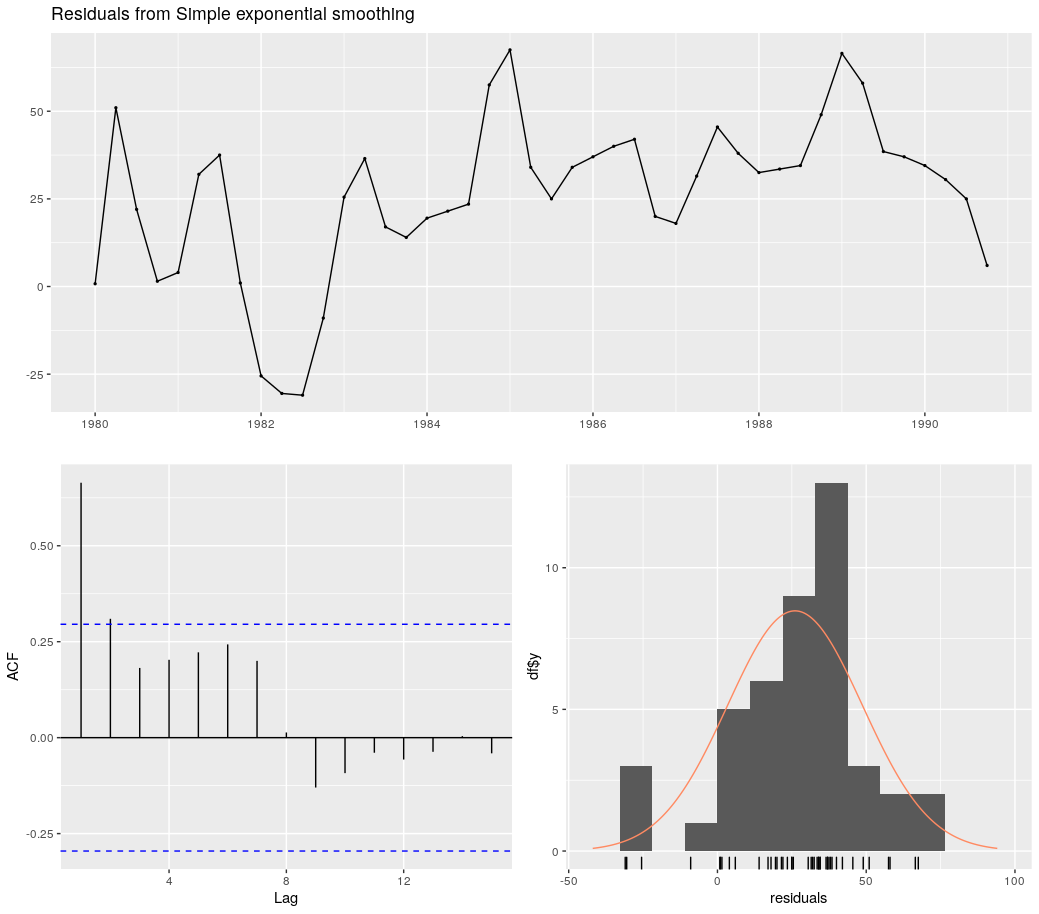
\includegraphics[width=\linewidth]{img/check_resid_ses.png}
  \caption{SES}
  \label{fig:ses_resid}
\end{subfigure}
\begin{subfigure}{.32\textwidth}
  \centering
  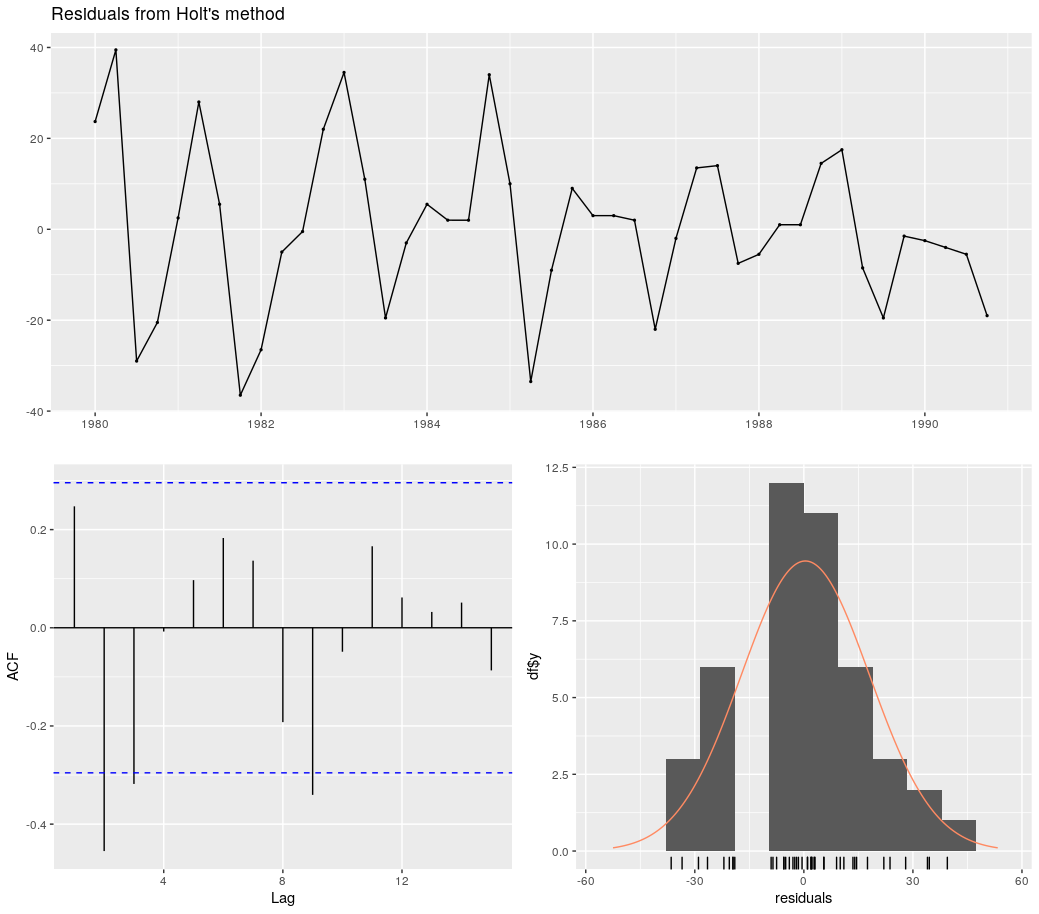
\includegraphics[width=\linewidth]{img/check_resid_holt.png}
  \caption{Holt}
  \label{fig:holt_resid}
\end{subfigure}
\begin{subfigure}{.32\textwidth}
  \centering
  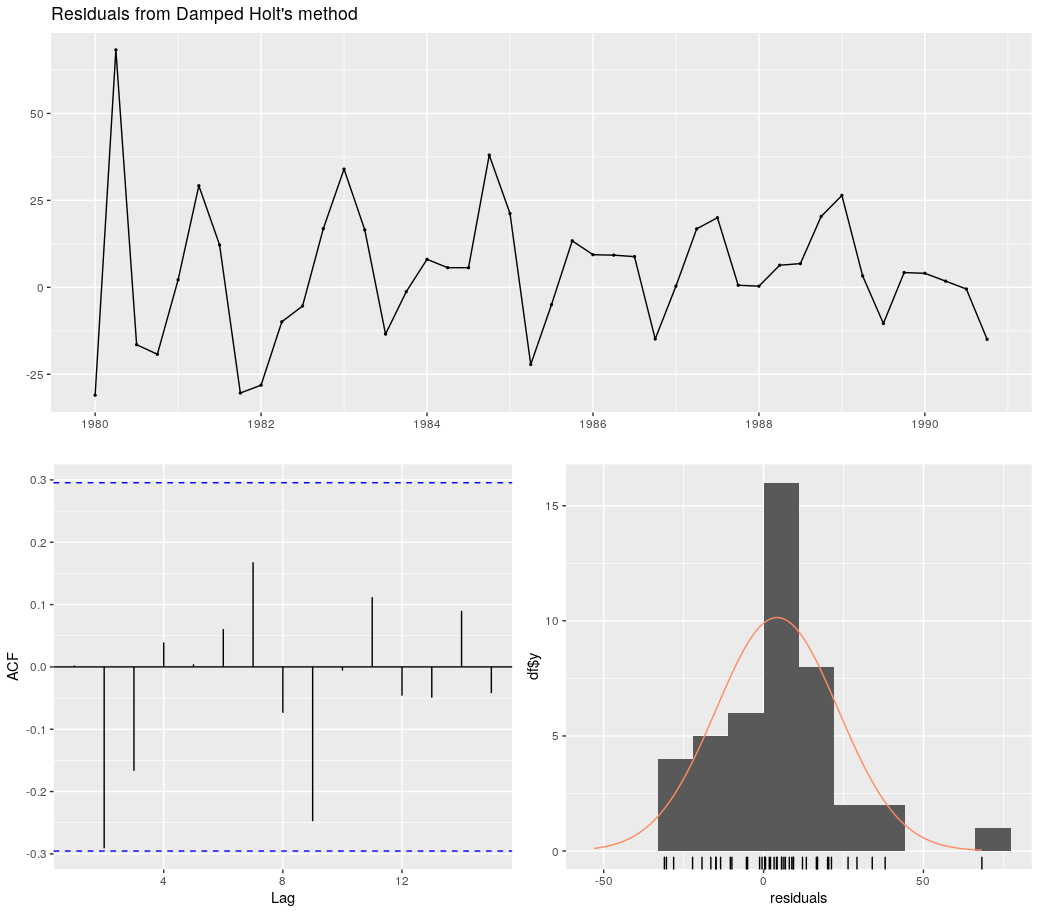
\includegraphics[width=\linewidth]{img/check_resid_holt_dampend.png}
  \caption{Holt's dampened}
  \label{fig:holt_d_resid}
\end{subfigure}
\caption{Checking residuals using multiple models}
\label{fig:exponential_smoothing}
\end{figure}



\begin{minipage}{.3\textwidth}
  \begin{lstlisting}[basicstyle=\tiny,numbers=none]
# Ljung-Box SES
data:  Residuals from Simple exponential smoothing
Q* = 37.012, df = 6, p-value = 1.751e-06

Model df: 2.   Total lags used: 8
\end{lstlisting}
\end{minipage}
\begin{minipage}{.3\textwidth}
  \begin{lstlisting}[basicstyle=\tiny,numbers=none]
# Ljung-Box Holt
data:  Residuals from Holt method
Q* = 23.215, df = 4, p-value = 0.0001147

Model df: 4.   Total lags used: 8
\end{lstlisting}

\end{minipage}
\begin{minipage}{.3\textwidth}
  \begin{lstlisting}[basicstyle=\tiny,numbers=none]
# Ljung-Box Holt dampened
data:  Residuals from damped Holt method
Q* = 7.5802, df = 3, p-value = 0.05553

Model df: 5.   Total lags used: 8
\end{lstlisting}
\end{minipage}
\captionof{lstlisting}{Listing of the three Ljung-Box tests}
\label{lst:threemodels}

\section{ETS and auto-ARIMA}
When we apply the \textit{ets} function in R, it returns as visible in \autoref{ets:output} an ETS(A,A,N) model, showing that the algorithm found a matching model with \textbf{additive error}, \textbf{additive trend} but without \textbf{seasonality}. It finds a linear holt model as the best performing for our dataset, even though the Ljung-Box test performs worse on the residuals.\newline
\begin{figure}[h]
\begin{minipage}{.6\textwidth}  %listing bloc will have 50% of the line width 
\lstset{linewidth = 6cm, breaklines=true} %set your listing lines widths, and set breaklines to true
\begin{lstlisting}[basicstyle=\footnotesize,numbers=none]
ETS(A,A,N) 
Call:
 ets(y = train) 
  Smoothing parameters:
    alpha = 0.9999 
    beta  = 0.9999 
  Initial states:
    l = 4601.9649 
    b = -12.1676 
  sigma:  18.2947
     AIC     AICc      BIC 
428.0925 429.6714 437.0134 

# Ljung-Box test
data:  Residuals from ETS(A,A,N)
Q* = 23.215, df = 4, p-value = 0.0001147

Model df: 4.   Total lags used: 8
\end{lstlisting}
\label{lst:ets}
\end{minipage}
\qquad %space between listing bloc and the figure
\begin{minipage}{0.6\textwidth} %figure will have the remaning 40% of the line width
    \centering
    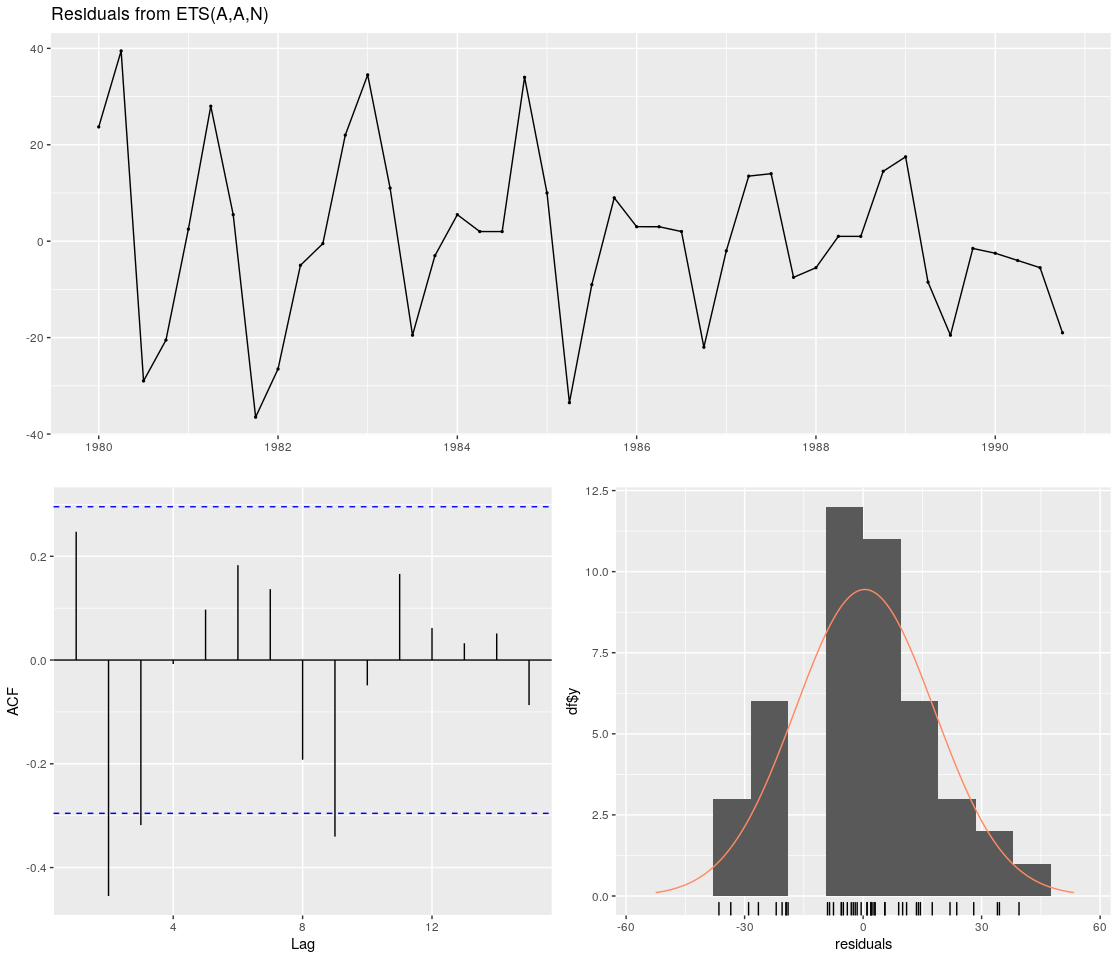
\includegraphics[width=0.9\textwidth]{img/check_resid_ets.png}
\end{minipage}
\caption{The output of the model analysis using ets}
\label{ets:output}
\end{figure}

Using the \textit{auto.arima} function in R, the algorithm finds an ARIMA(0,2,1) model, giving no auto regressive part, 2 differences, and a moving average of order 1 but without seasonality. The residuals in \autoref{fig:arima_analysis} seem to be better distributed, the ACF plot has less autocorrelation visible but the Ljung-Box test still performs worse, with a p-value of 0.01, which is less then the chosen threshold of 5\%.
\clearpage
\begin{figure}[ht!]
\begin{minipage}{.6\textwidth}  %listing bloc will have 50% of the line width 
\lstset{linewidth = 6cm, breaklines=true} %set your listing lines widths, and set breaklines to true
\begin{lstlisting}[basicstyle=\footnotesize,numbers=none]
ARIMA(0,2,1) 
Coefficients:
         ma1
      0.7537
s.e.  0.0986

sigma^2 = 179.4:  log likelihood = -168.37
AIC=340.74   AICc=341.04   BIC=344.21

# Ljung-Box test
data:  Residuals from ARIMA(0,2,1)
Q* = 17.661, df = 7, p-value = 0.0136
Model df: 1.   Total lags used: 8
\end{lstlisting}
\end{minipage}
\qquad %space between listing bloc and the figure
\begin{minipage}{0.6\textwidth} %figure will have the remaning 40% of the line width
    \centering
    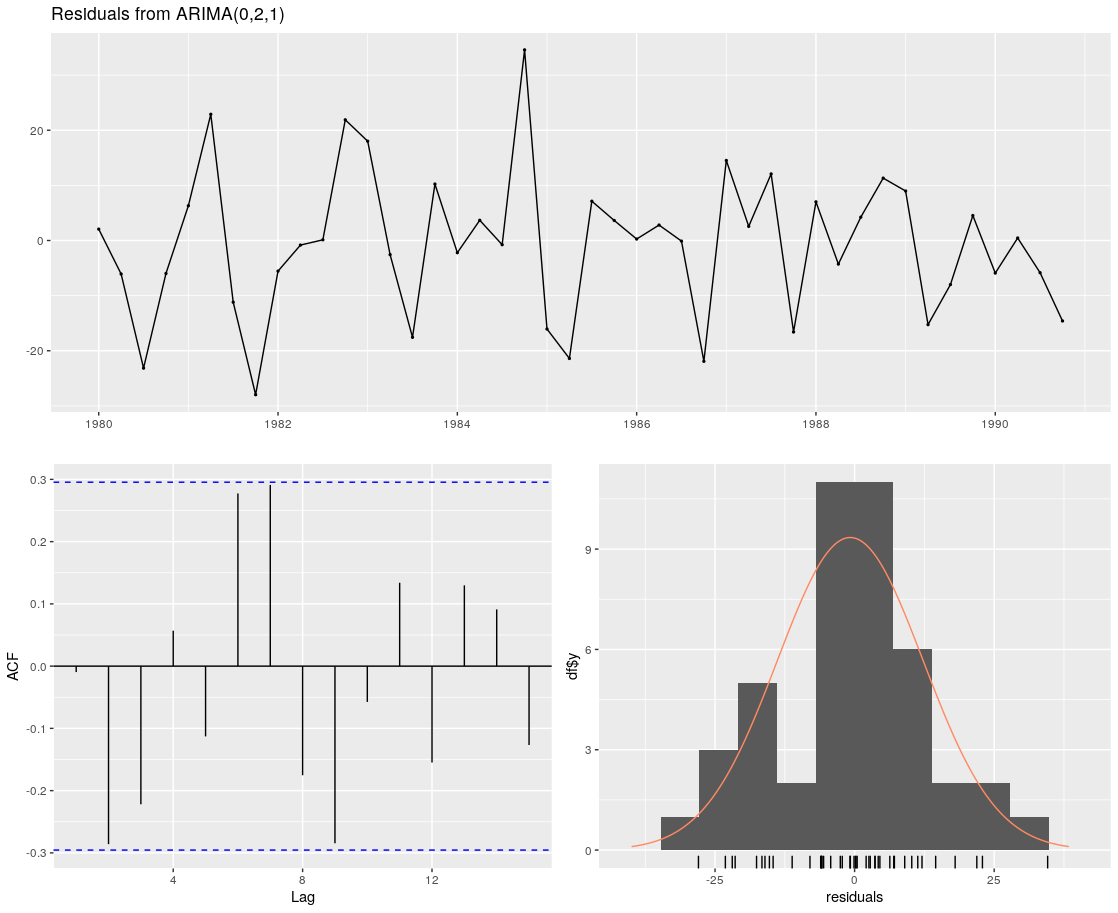
\includegraphics[width=0.8\textwidth]{img/check_resid_auto_arima.png}
\end{minipage}
\caption{Output of the analysis using auto.arima}
\label{fig:arima_analysis}
\end{figure}
\section{Conclusion}
The chosen time series is typical for stock or other economy related series. For this reason, good predictions are quite hard to achieve. All models tested had difficulties predicting our test data. The only model where the p-value indicated that the residuals are white noise is Holt's dampened model. But when looking at the results for our chosen indicators in \autoref{tab:holt_d_accuracy} we see that the found Arima model is clearly the best. This becomes even clearer when looking at \autoref{fig:forecast_holt_dampend}. It is followed by SES and Holt's linear model which still both fulfill our set targets for the indicators. For these reasons, we were able to be better than our set targets but we also have learned that in time series prediction all metrics and values must be taken into account in order to find the best model. Furthermore, we would suggest using cross-validation for further investigations to find the best model.
\begin{figure}[ht!]
    \centering
    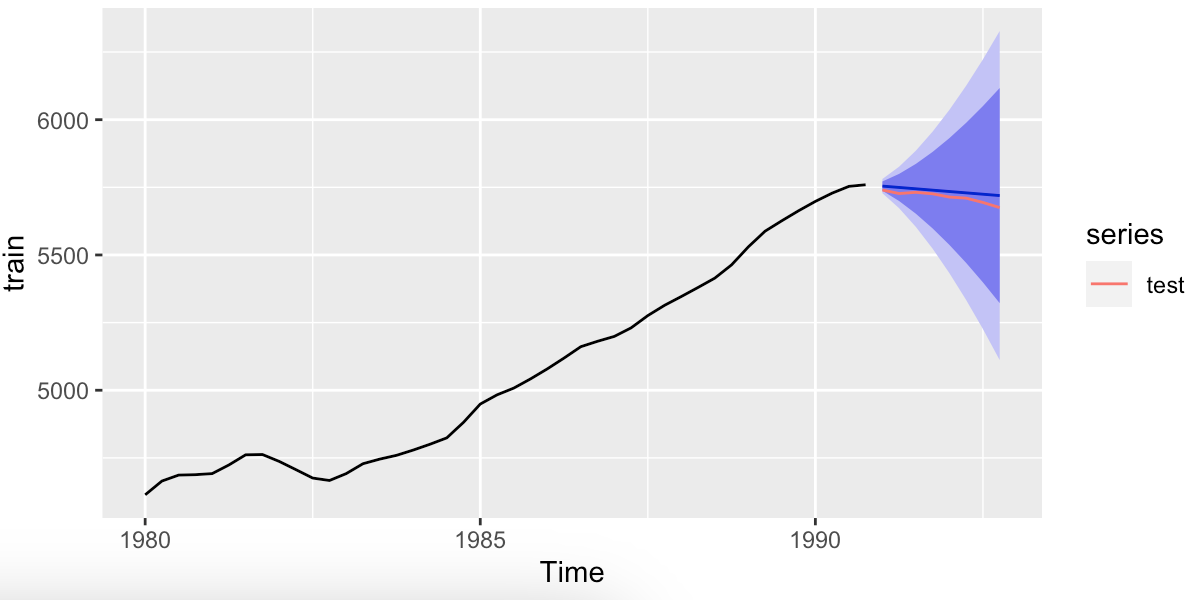
\includegraphics[width=0.8\textwidth]{img/forecast_arima.png}
    \caption{Forecast with ARIMA(0,2,1) model}
    \label{fig:forecast_holt_dampend}
\end{figure}



\begin{table}[h]
\small
\centering
\begin{tabular}{cccccccc}
  \hline
 Indicator & Set & RW w. drift & SES & Holt\'s linear & Holt\'s dampened & ETS(A,N,N) & Auto Arima (0,2,1)  \\ 
  \hline
\multirow{2}{*}{RMSE} & Train & 22.32  & 34.37 & 17.44 & 19.34 & 17.44 & 12.93 \\ 
  & Test & 100.96 & 28.91 & 44.87 & 67.17 & 79.20 & 24.44 \\
  \hline 
  \multirow{2}{*}{MAE} & Train &  16.69 & 30.43 & 13.16 & 14.39 & 13.16 & 9.84 \\ 
  & Test & 95.00 & 28.37 & 43.38 & 61.97 & 71.82 & 22.31 \\ 
   \hline
\end{tabular}
\caption{Accuracy the different trained models}
\label{tab:holt_d_accuracy}
\end{table}
\clearpage
%\printbibliography[title={Bibliography}]

\printbibliography

\end{document}
